%% For boldface greek letters:
\def\bmath#1{\mbox{\boldmath$#1$}} 


\section{Angular Momentum and Torque as Vectors\footnote{
1990-93 Dept. of Physics and Astronomy, Dickinson College. Supported by FIPSE
(U.S. Dept. of Ed.) and NSF. Portions of this material may have been modified
locally and may not have been classroom tested at Dickinson College.
}}

Name \rule{2.0in}{0.1pt}\hfill{}Section \rule{1.0in}{0.1pt}\hfill{}Date \rule{1.0in}{0.1pt}

Objectives 

To understand the definitions of torque and angular momentum as vector quantities
and to understand the mathematical properties and some applications of the vector
cross product. We will also learn the relationship between torque and angular
momentum.

\textbf{Apparatus}

\begin{itemize}
\item A horizontal pivot
\item Vertical rod for horizontal pivot (mounted on table edge)
\item Spring scale (5 newton)
\item A ruler 
\item A protractor 
\item Rods and connectors (Styrofoam ball and bamboo skewers)
\item Two small masses (100g \& 200g) 
\item A Rotating Disk System 
\item String and pulley (with mountin clamp)
\end{itemize}
\textbf{Overview} 

This unit presents us with a consolidation and extension of the concepts in
rotational motion that you have studied so far. You studied the analogy and
relationships between rotational and linear quantities (i.e., position and angle,
linear velocity and angular velocity, linear acceleration and angular acceleration,
and force and torque) without taking into account, in any formal way, the fact
that these quantities actually behave like the mathematical entities we call
vectors. We will discuss the vector nature of rotational quantities and, in
addition, define a new vector quantity called angular momentum that is the rotational
analog of linear momentum. 

Angular momentum and torque are special vectors because they are the product
of two other vectors a position vector and a force or linear momentum vector.
To describe them we need to introduce a new type of vector product known as
the vector cross product. We will explore the definition and unique nature of
the vector cross product used to define torque and angular momentum. We will
study the relationship between torque and angular momentum as well as the theoretical
basis of the Law of Conservation of Angular Momentum.

\textbf{Observation of Torque when \( {\bf F} \) and \( {\bf r} \)
are not Perpendicular} 

Recently, you ``discovered'' that if we define torque as the
product of a lever arm and perpendicular force, an object does not rotate when
the sum of the torques acting on it add up to zero. However, we didn't consider
cases where \textbf{\( {\bf F} \)} and \textbf{\( {\bf r} \)}
are not perpendicular, and we didn't figure out a way to tell the direction
of the rotation resulting from a torque. Let's consider these complications
by generating torques as described below.

\textbf{Activity 1: Torque as a Function of Angle} 

(a) Suppose you were to hold one of the forces in the following figure (which is a TOP view of the horizontal pivot) at an angle of 90\( ^{\circ } \)
with respect to the lever arm, \( r_{h} \), and pull on it with a steady force.
This can be done by attaching a string to the left side of the horizontal pivot, placing the string over a mounted pulley, and hanging a 200g mass on the string. Meanwhile you can attach a scale to the other end of the pivot and pull on it at several angles other than 90\( ^{\circ } \)
from its lever arm, \( r_{app} \), as shown in the figure. Would the magnitude of the balancing force be less than, greater than, or equal to the force needed at 90\( ^{\circ } \)? What do you predict? Explain. (Remember, this figure is a TOP view. Both forces in the figure should be HORIZONTAL.)

\vspace{0.3cm}
{\par\raggedright 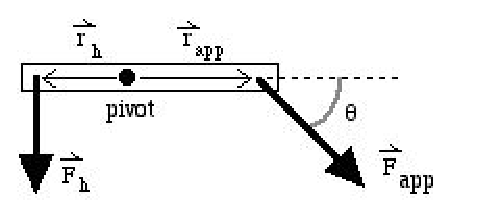
\includegraphics{ang_mom_fig1.eps} \par}
\vspace{0.3cm}

(b) You should determine exactly how the forces compare to that needed at a
90\( ^{\circ } \) angle. Determine this force for at least four different angles
and figure out a mathematical relationship between $F$, $r$, and \( \theta  \).
Set up a spreadsheet to do the calculations shown in the table below. Hint:
Should you multiply the product of the measured values of $r$ and $F$ 
by sin \( \theta  \)
or by cos \( \theta  \) to get a torque that is equal in magnitude to the holding
torque?

\vspace{0.3cm}
{\centering \begin{tabular}{|c|c|c|c|c|c|c|c|c|c|}
\hline 
\( r_{h} \)&
\( F_{h} \)&
\( \tau _{h} \)&
\( r_{app} \)&
\( F_{app} \)&
\( \theta  \)&
\( \cos \theta  \)&
\( \sin \theta  \)&
\( r_{app} F_{app}\cos \theta  \) &
\(r_{app} F_{app}\sin \theta  \)\\
(m)&
(N)&
(N m)&
(m)&
(N)&
(deg)&
&
&
(N m)&
(N m)\\
\hline 
\hline 
&
&
&
&
&
&
&
&
&
\\
&
&
&
&
&
&
&
&
&
\\
\hline 
&
&
&
&
&
&
&
&
&
\\
&
&
&
&
&
&
&
&
&
\\
\hline 
&
&
&
&
&
&
&
&
&
\\
&
&
&
&
&
&
&
&
&
\\
\hline 
&
&
&
&
&
&
&
&
&
\\
&
&
&
&
&
&
&
&
&
\\
\hline 
&
&
&
&
&
&
&
&
&
\\
&
&
&
&
&
&
&
&
&
\\
\hline 
\end{tabular}\par}
\vspace{0.3cm}

(c) Within the limits of uncertainty, what is the most plausible mathematical
relationship between \( \tau  \) and $r$, $F$, and \( \theta  \)?
\vspace{20mm}

The activity you just completed should give you a sense of what happens to the
magnitude of the torque when the pulling force, \( {\bf F} \), is
not perpendicular to the vector, \( {\bf r} \), from the axis of
rotation. But how do we define the direction of the rotation that results when
the torque is applied to an object that is initially at rest and not balanced
by another torque? Let's consider the directions we might associate with angular
velocity and torque in this situation.

\textbf{Activity 2: Angular Rotation, Torque, and Direction }

(a) Suppose a particle is moving around in a circle with an angular velocity
that has a magnitude of \( \omega  \) associated with it. According to observer
\#1, does the particle appear to be moving clockwise or counter clockwise? How
about the direction of the particle's motion according to observer \#2?

\vspace{0.3cm}
{\par\raggedright 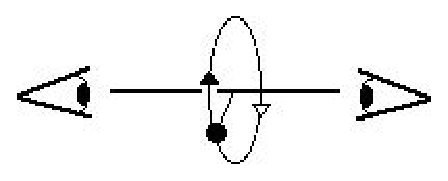
\includegraphics{ang_mom_fig2.eps} \par}
\vspace{0.3cm}

(b) Is the clockwise vs. counterclockwise designation a good way to determine
the direction associated with $\omega$ in an unambiguous way? Why or why not? 
\vspace{20mm}

(c) Can you devise a better way to assign a direction to an angular
velocity?
\vspace{20mm}

(d) Similar consideration needs to be given to torque as a vector. Can you devise
a rule to assign a direction to a torque? Describe the rule.
\vspace{20mm}

\textbf{Discussion of the Vector Cross Product }

An alternative to describing positive and negative changes in angle is to associate
a directed vector with the axis of rotation using an arbitrary but
well accepted rule called the right-hand rule. By using vectors we can describe
separate rotations of many body systems all rotating in different planes about
different axes. 

By using this vector assignment for direction, angular momentum and torque can
be described mathematically as ``vector cross products.'' The
vector cross product is a very strange type of vector multiplication worked
out many years ago by mathematicians who had never even heard of angular momentum or torque. The peculiar properties of the vector cross product and its relationship to angular momentum and torque are explained in most introductory physics textbooks.
The key properties of the vector that is the cross product of two vectors \( 
{\bf r} \)
and \( {\bf F} \) are that:

\begin{enumerate}
\item The magnitude of the cross product is $rF\sin\theta$ where \( \theta  \)
is the angle between the two vectors; 
\[
\left| {\bf r}\times {\bf F}\right| =\left| {\bf r}\right| \left| {\bf F}\right| \sin \theta .\]
The term \( \sin \theta  \) picks out the component of \( {\bf F} \)
along a line perpendicular to \( {\bf r} \).
\item The cross product of two vectors \( {\bf r} \) and \( {\bf F} \)
is a vector that lies in a direction perpendicular to both \( {\bf r} \)
and \( {\bf F} \) and is up if \( {\bf F} \) causes
a counter-clockwise rotation, and is down if \( {\bf F} \) causes
a clockwise rotation. These properties of the cross product are pictured below.
\end{enumerate}
\vspace{0.3cm}
{\par\centering 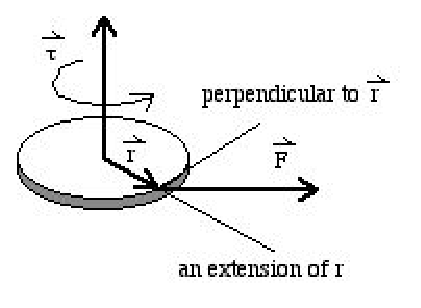
\includegraphics{ang_mom_fig3.eps} \par}
\vspace{0.3cm}

The spatial relationships between \( {\bf r} \), \( {\bf F} \),
and \( {\bmath{\tau} } \) are very difficult to visualize. In the next
activity you can connect some thin rods of various sizes to each other at angles
of your own choosing and make some ``vector cross products.''

\textbf{Activity 3: Making Models of Vector Cross Products} 

(a) Pick out rods of two different lengths and connect them at some angle you
choose. Consider one of the rods to be the \( {\bf r} \) vector
and the other to be the \( {\bf F} \) vector. Measure the angle
\( \theta  \) and the lengths of \( {\bf r} \) and \( {\bf F} \)
in meters. Then compute the magnitude of the cross product as 
$rF\sin \theta $
in newton meters (N m). Show your units! Note: You should assume that the magnitude
of the force in newtons is represented by the length of the rod in meters.
\vspace{20mm}

(b) Attach a ``cross product'' rod perpendicular to the plane
determined by \( {\bf r} \) and \( {\bf F} \) with a
length of $rF\sin \theta$. Sketch the location of \( {\bf F} \)
relative to \( {\bf r} \) in the space below. Show the direction
and magnitude of the resultant torque \( {\bmath{\tau} } \). \textit{Finally,
show your cross product model to an instructor or fellow student for confirmation
of its validity. }

\vspace{0.3cm}
{\par\centering 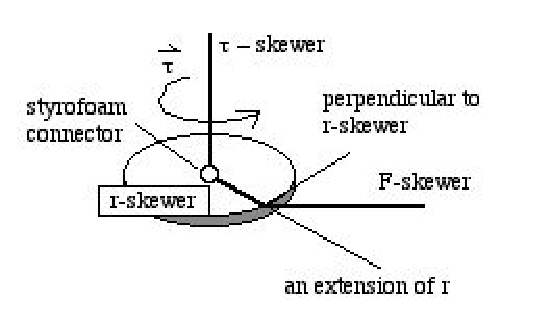
\includegraphics{ang_mom_fig4.eps} \par}
\vspace{0.3cm}

\textbf{Figure 2: A Model of the Vector Cross Product}

(c) In the diagrams below the vectors \( {\bf r} \) and \( {\bf F} \)
lie in the plane of the paper. Calculate the torques for the following two sets
of \( {\bf r} \) and \( {\bf F} \) vectors. In each
case measure the length of the \( {\bf r} \) vector in meters and
assume that the length of the \( {\bf F} \) vector in cm represents
the force in newtons. Use a protractor to measure the angle, \( \theta  \),
between the extension of the \( {\bf r} \)-vector and the \( {\bf F} \)-vector.
Calculate the magnitude of the torques. Place the appropriate symbol to indicate
the direction of the torque in the circle as follows: a circle with an x in
it indicates a vector into the page, while a circle with a dot in it indicates
a vector out of the page.

\vspace{0.3cm}
{\par\centering 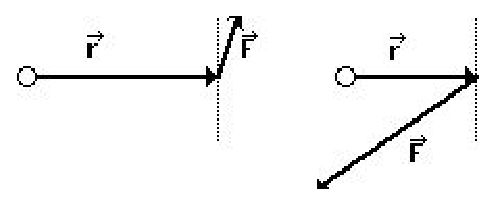
\includegraphics{ang_mom_fig5.eps} \par}
\vspace{0.3cm}

$r =$ \rule{0.5in}{0.1pt} m \hfill{}$F =$ 
\rule{0.5in}{0.1pt} N \hfill{}\( \theta  =\)
 \rule{0.5in}{0.1pt} \hfill{}\( \tau  =\)  \rule{0.5in}{0.1pt} N\( \cdot  \)m 
\vspace{5mm}

$r = $\rule{0.5in}{0.1pt} m \hfill{}$F =$ \rule{0.5in}{0.1pt} N \hfill{}
\( \theta = \)
\rule{0.5in}{0.1pt} \hfill{}\( \tau  =\)  \rule{0.5in}{0.1pt} N\( \cdot  \)m
\vspace{5mm}

\textbf{Momentum and its Rotational Analog} 

Once we have defined the properties of the vector cross product, another important
rotational vector is easily obtained, that of angular momentum relative to an
axis of rotation. 

\textbf{Activity 4: Angular and Linear Momentum }

(a) Write the rotational analogs of the linear quantities shown. Note: Include
the formal definition (which is different from the analog) in spaces marked
with an asterisk ({*}). For example the rotational analog for velocity is angular velocity \( \bmath{\omega}  \) and the definition of its magnitude is \( |
\bmath{\omega}  |
= d \theta  /dt\) rather than $v/r$.

\vspace{0.3cm}
{\centering \begin{tabular}{|p{5cm}|p{5cm}|p{5cm}|}
\hline 
Linear Quantity&
Rotational Quantity&
Definition\\
\hline 
\hline 
&
&
\\
$x$ (position) &
&
\\
\hline 
&
&
{*}\\
$v$ (velocity) &
&
\\
\hline 
&
&
{*}\\
$a$ (acceleration) &
&
\\
\hline 
&
&
{*}\\
$F$ (Force) &
&
\\
\hline 
&
&
{*}\\
$m$ (mass) &
&
\\
\hline 
&
&
\\
$F = ma$&
&
\\
\hline 
\end{tabular}\par}
\vspace{0.3cm}

(b) What do you think will be the rotational definition of angular momentum
in terms of the vectors \( {\bf r} \) and \( {\bf p} \)?
\textbf{Hint:} This is similar mathematically to the definition of torque and
also involves a vector cross product. (Note that the symbol for angular momentum is \textbf{L}).
\vspace{20mm}

(c) What is the rotational analog in terms of the quantities $I$ and \( 
\bmath{\omega}  \)? (This is analogous to \textbf{p} = m\textbf{v}.)
Do you expect the angular momentum to be a vector? Explain.
\vspace{30mm}

\textbf{Torque and Change of Angular Momentum }

Earlier in this course you applied a very brief force along a line through the
center of mass of a rolling cart. Do you remember how it moved? What happened
when you applied a gentle but steady force along a line through the center of
mass of the cart? Let's do analogous things to a disk that is free to rotate
on a relatively frictionless bearing, with the idea of formulating laws for
rotational motion that are analogous to Newton's laws for linear motion. 

Figure out how to use a system like that shown in the figure below to observe
the motion of the disk under the influence of a brief torque and a steady torque.
In describing the Laws of Rotational Motion be sure to consider vector properties
and take both the magnitudes and directions of the relevant quantities into
account in your wordings. 

\vspace{0.3cm}
{\par\centering 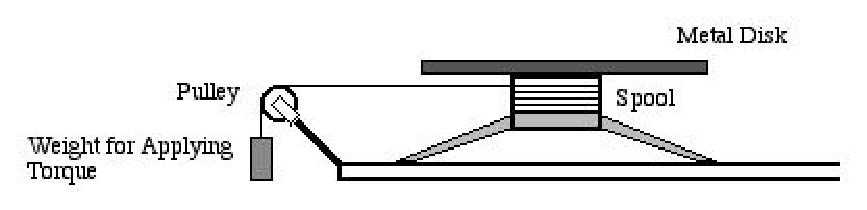
\includegraphics{ang_mom_fig6.eps} \par}
\vspace{0.3cm}

\textbf{Activity 5: Applied Torques and Resultant Motion }

(a) After applying a brief torque and then removing the torque, what happens to the angular velocity and hence the angular momentum of the
disk? State a First Law of Rotational Motion in terms of torques and angular momenta. \textbf{Hint:} Newton's first law in translational form states that the center of mass of a system of particles or a rigid object that experiences no net external force will experience no change in linear momentum and so will continue to move at constant velocity.

Newton's First Law in rotational form (in words):
\vspace{20mm}

Newton's First law in rotational form as a mathematical expression: 
\vspace{20mm}

(b) What happens to the magnitude and direction of the angular velocity (and
hence the angular momentum) of the disk during the application of a steady torque? How do they change relative to the magnitude and direction of the torque? If
possible, give a precise statement of a Second Law of Rotational Motion relating the net torque on an object to its change in angular momentum. \textbf{Note:}
Take both magnitudes and directions of the relevant vectors into account in
your statement. \textbf{Hint}: Newton's second law of motion in translational form states that if the center of mass
of a system of particles or rigid object experiences a net external force, it 
will undergo a change in linear momentum such that the rate of change of linear momentum is equal to the net force.

Newton's Second Law of Rotational Motion (in words):
\vspace{20mm}

Newton's Second Law of Rotational Motion as a Vector Equation:
\vspace{20mm}

\textbf{Angular Momentum Conservation }

Now use the vector expression for Newton's Second Law of Rotational
Motion to show that, in theory, we expect angular momentum on a system to be
conserved if the net torque on that system is zero.

